% 20200719
\documentclass[../thesis.tex]{subfiles} %% use packages & commands as this main file
\begin{document}
\section{Result}
\Phy-only (\PoH\ and \PoN) systems yielded significantly higher than their coexisting (\PBH\ and \PBN) versions in selected harvest modes and values (Fig.\ref{f:ydByHarv}, p$\ll$0.01).  Regardless of harvest rates/intervals, \phy-only systems did not have significant difference (p $>$ 0.1) in log yields (Fig.\ref{f:ydByHarv}).

Log distributions for \phy-only systems were stable with much wider yield ranges than \pbs\ regardless of harvest mode (Fig.\ref{f:ydByHarv}).  On a contrary, most \pbs s yielded 0 \dxdt\ (for both medians and interquartile ranges) with an exception of \PBN\ systems with low harvest interval (median 0.02, IQR [-0.01 - 0.12]\dxdt).  For maximum yield scenarios of each of the four systems, \PoH\ and \PoN\ have similar yield of 345-346\dxdt.  \PBH\ systems had an overall decreased yet fluctuating maximum from 275 ($x$ = 101) to 176 ($x$ = 1001) to 218 ($x$ = 10001) \dxdt.  \PBN systems had a decreased and flattened maximum trend from 198 ($x$ = 101) to 66 ($x$ = 1001 and 10001) \dxdt.

Pairwise Wilcox test showed statistical significance for all four systems (\PBH, \PoH, \PBN\ \& \PoN).  Yet in Fig.\ref{f:ydByPara} the pair of \phy-only systems were largely overlapping and the overlap was also observed for the \pbs s.  Hence we concluded that biological significance was only between \phy-only and \pbs s but not across harvest terms within each pair.

Biological parameters for \phy\ (Fig.\ref{f:ydByPara}A-D) had stable influence over \phy-only systems (\PoH\ \& \PoN) in the view of the median.  No parameters had influence on median values for \pbs s (\PBH\ \& \PBN in Fig.\ref{f:ydByPara}A-H).  As for \phy\ biological parameters, only intraspecific interference ($\aP$) had a decreasing effect in a decreasing rate.  Hence density-insensitive \phy\ death rate had much higher productivity than others; maximum yield for all four systems concentrated at the minimal value for this parameter range.  The other three \phy\ parameters (i.e. non-respirable carbon fraction for \phy\ $\ePR$, carbon fraction allocated into biomass for \phy\ $\eP$ and \phy\ growth rate $\gP$) had a stable positive influence on median of \phy-only systems yield fluxes.  Although pairwise Wilcox test showed significance (p $\ll$ 0.01) between \PoH\ and \PoN, the difference may not be biological significant.  The set of four parameters had no observational effect on \pbs s.  The reason was because most of the raw yield from simulations were zeros.  Details were listed later in this section.

Biological parameters for \bac\ (Fig.\ref{f:ydByPara}E-H) had no observable influence over all systems.  It had no effect on \phy-only systems mathematically (equilibrium 3 in Table \ref{t:eqm}).  Hence fluctuations from \phy-only systems in Fig.\ref{f:ydByPara}E-H was due to LHS sampling effect.  It also had no observational effect on 

\begin{figure}[H]
    \centering
    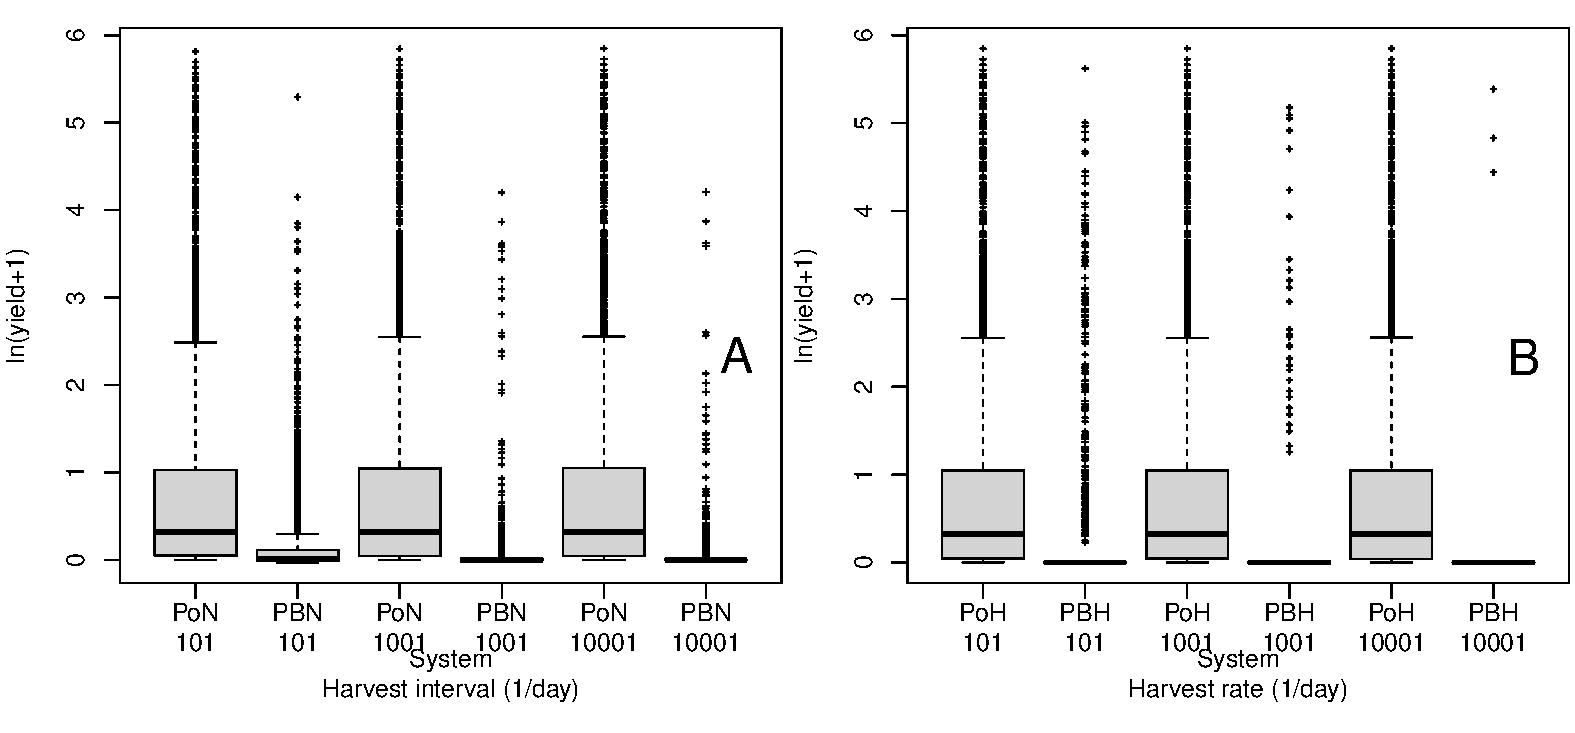
\includegraphics[width=\linewidth]{result/Harvest.pdf}
    \caption[Yield flux distribution by harvest mode]{Log distribution of yield for destructive (subplot A) and continuous (subplot B) harvest modes on selected harvest interval/rates.  For both subplots, pairwise Wilcox test showed significance between \phy-only (\PoH/\PoN) and coexistence (\PBH/\PBN) systems (p $\ll$ 0.01), between harvest rates/intervals within the group of \pbs s (p $\ll$ 0.01) but not \phy-only systems (p $>$ 0.1).  Each box represented a sample size of 5500.}
    \label{f:ydByHarv}
\end{figure}

\begin{figure}[H]
    \centering
    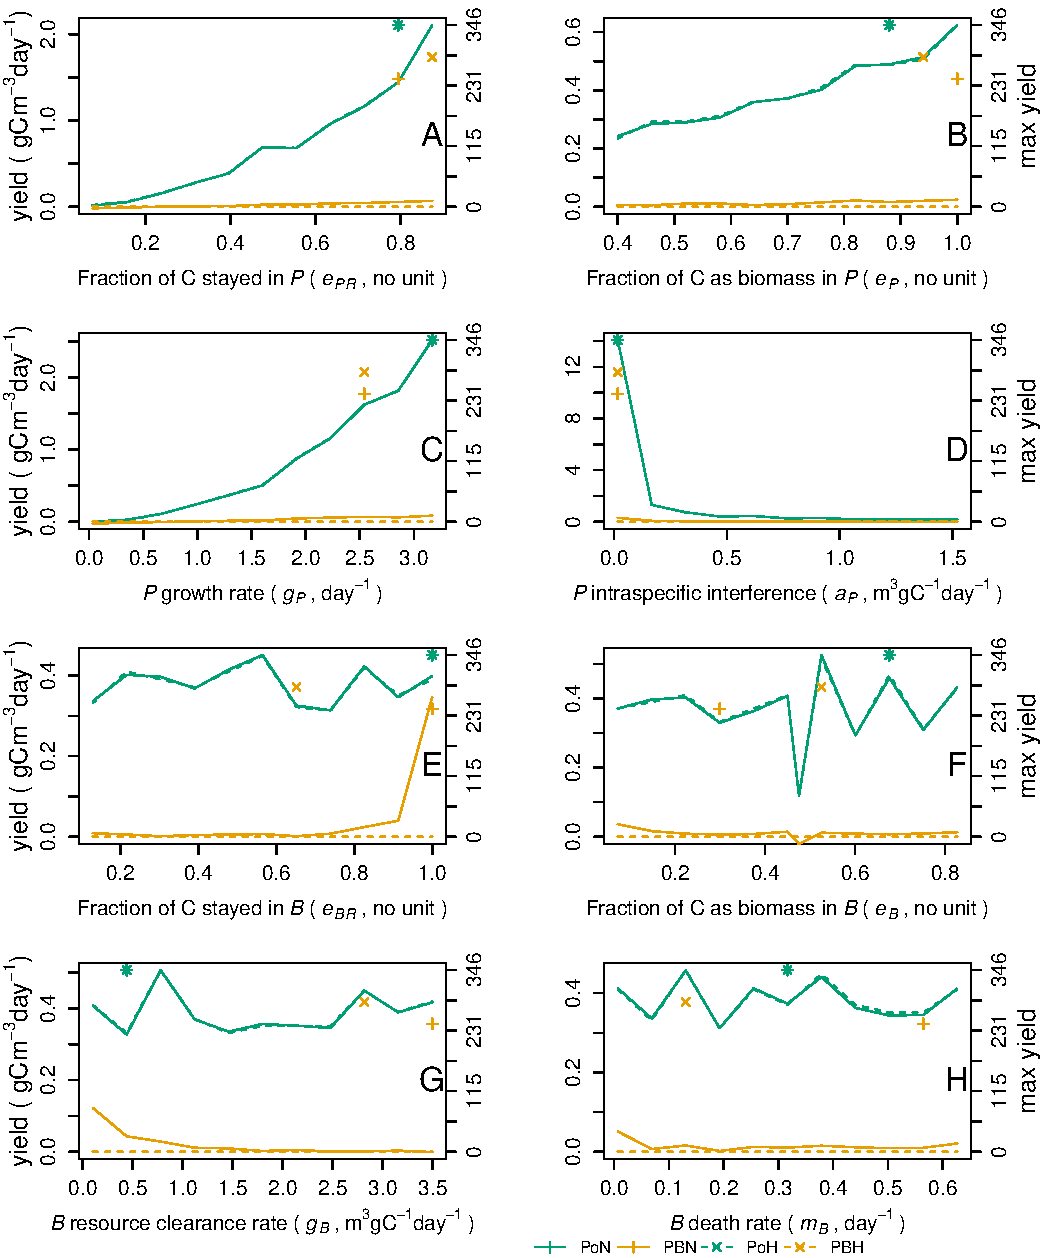
\includegraphics[width=\linewidth]{result/yieldFlux.pdf}
    \caption[Yield flux median in biological parameter space]{Median yield flux (primary axis) and the maximum yield scenario (secondary axis) along respective parameter ranges under a standardised temperature range of \temp.  Each system had an LHS sample size of 1.1 million.  Pairwise Wilcox test showed significance (p $\ll$ 0.01) between all systems.}
    \label{f:ydByPara}
\end{figure}

\end{document}